\chapter{Experiment and Evaluation}

\section{Experimental Settings}
In this section, we describe the general experimental settings applied to all the following experiments, for different experiments, their additional settings will be described in corresponding sections. For the fairness, all the evaluation are eventually conducted on the pre-processed ``raw'' data without any futher transformation. This decision is made because of the facts: (1)
different represent methods generate varying number of features, and the number of features will affect the computation of indexes listed in Section~\ref{sec:metrics}; (2) the separation quality could be good on the transformed data, but may not also acceptable on the original data, in term of the trend analysis, the latter one is more important. 

\subsection{Numerical Metrics}
\label{sec:metrics}
Generally, there are two indexes to evaluate the quality of data groups. The first one is the external index, it requires additional ground truth information to compare the generated groups with a reference model. Our dataset dose not contain such information, and hence the metric used here is the \textbf{internal index}. Literally, internal index reveals the intrinsic attributes of the groups, and does not require reference model. The common internal indexes are:
\begin{enumerate}
    \item Silhouette Coefficient (SC) \cite{rousseeuw1987silhouettes}: for each data point, its silhouette coefficient is composed of two scores:
    \begin{itemize}
        \item \textbf{a:} the average distance between a data point and all other data points in the same cluster
        \item \textbf{b:} the average distance between a data point and all other data points in the next nearest cluster
    \end{itemize}
    The Silhouette Coefficient s for a single data point is defined as follows, where s ranges from -1 to +1:
    \begin{equation}
        s = \frac{b-a}{\max(a,b)} 
    \end{equation}
    The final Silhouette Coefficient is defined as the mean of the Silhouette Coefficient of each data point. \textbf{Higher Silhouette Coefficient Index means better clustering results}.
    \item Calinski-Harabasz (CH) Index \cite{calinski1974dendrite}: given a data set E of size $n_E$, and the number of grouped clusters k, the Calinski-Harabasz score s is defined as follows:
    \begin{equation}
        s = \frac{tr(B_k)}{tr_(W_k)} \times \frac{n_E - k}{k-1}
    \end{equation}
    \begin{equation}
        W_k = \sum_{q=1}^k \sum_{x \in C_q}(x-c_q)(x-c_q)^T
    \end{equation}
    \begin{equation}
        B_k = \sum_{q=1}^k n_q(c_q-c_E)c_q-c_E)^T
    \end{equation}
    Where $tr(B_k)$ and $tr(W_k)$ are trace of the between group dispersion matrix and within-cluster dispersion matrix respectively, $C_q$ represents the points in cluster $q$, $c_q$ represents the centre of $q$, $c_E$ represents the centre of E and $n_q$ represents the number of points in q. \textbf{Higher Calinski-Harabasz Index means better clustering results}.
    \item Davies-Bouldin (DB) Index \cite{davies1979cluster}: given two cluster $C_i$ and $C_j$ generated from the same data set without overlapping, their similarity $R_{ij}$ is defined as follows:
    \begin{equation}
        R_{ij} = \frac{s_i + s_j}{d_{ij}}
    \end{equation}
    Where $s_i$ is the average distance between each point in cluster $i$ and the centroid of $i$, $d_{ij}$ is the distance between centroids of clusters $i$ and $j$. The Davies-Bouldin index is defined as:
    \begin{equation}
        DB = \frac{1}{k} \sum_{i=1}^k\max_{i\neq j}R_{ij}
    \end{equation}
    k is the number of clusters. \textbf{Lower Davies-Bouldin index means better clustering results}.
\end{enumerate}
In the context of stock grouping analysis, analysts usually expect compact groups, especially when there is no explicit class information (the labels), because compact groups can reveal more general trends. In this aspect, these three indexes is relatively informative. Note that since they focus on different aspects, their trends may not comply with each other, but in general, if a grouping result gets high mark on all the three indexes, it can be regarded as a good separation.

\subsection{Measures to counteract the effect of randomness}
One well-known fact about clustering algorithms is that their outputs.

\subsection{The choice of group centers}
The generated groups could be mess, and it is necessary to highlight their centers when analyse their trends. One simplest way to extract the representative in a group is computing the arithmetic mean of that group. This method is called Euclidean Barycenter, it minimize the summed euclidean distance of that group. However, this method may be inappropriate in this project, since we will visualize the results with the original sequences, and the original data are not aligned. This is illustrated in Figure~\ref{fig:barycenter1}, where the red lines represent the computed centers and black lines represent the data points in the group. To better reveal the general trend of a group, we use the Dynamic Time Warping (DTW) based method to compute the barycenter. As mentioned before, DTW is a distance measure that can be used to compare two un-aligned sequences. Since it uses the dynamic programming, its time complexity is $O(mn)$, where $m$ and $n$ are the length of that two sequences respectively. To reduce the time complexity, we use its variation ``Soft-DTW'' to compute the center. The computation details of Soft-DTW can be found in \cite{schultz2018nonsmooth}. The second row of the figure shows the center computed by Soft-DTW with $\gamma$ set to 1, compared with the Euclidean barycenter, this center is visually more representative. 
\begin{figure}[!htbp]
    \centering
    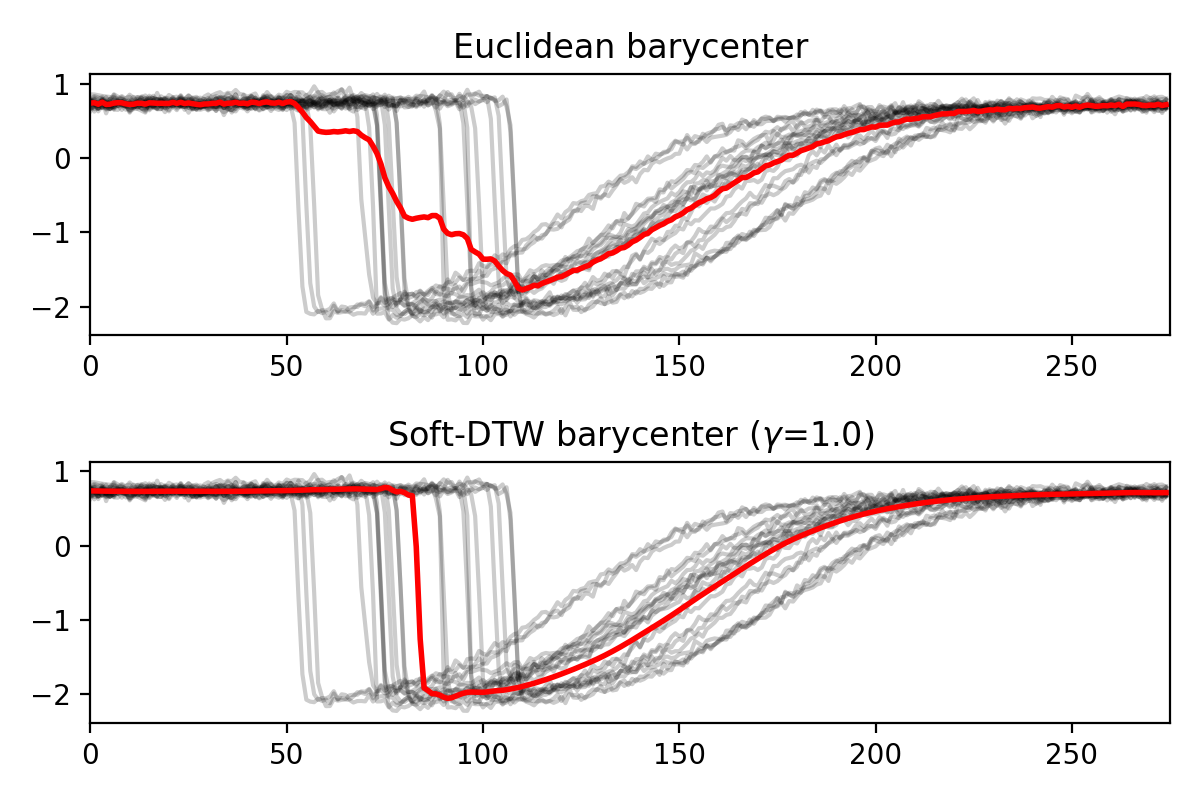
\includegraphics[width=0.6\columnwidth]{barycenter.png}
    \caption{Barycenter}
    \label{fig:barycenter1}
\end{figure} 


\section{Comparison of PIP, PAA and Down Sampling}
In Section~\ref{sec:pippaa}, we use the similarity measures with visually similar stocks to evaluate the perfomance of three different sequence compression methods, and find that these three methods show no significant difference in terms of such measurement. However, as mentioned before, some compression methods can preserve key points while others can not, we believe this functionality does affect the final perfomance of some applications. Besides, we persume that the global scaling invariance and occlusion invariance can be partially achieved by sequence reduction and approximation. Therefore, we decide to add this section to evaluate and verify the effectiveness of these three compression algorithms in the context of time series clustering task. The test data used here are the records of all stocks in our dataset. The number of clusters is limited up to 15 to tradeoff of the ease of visualization and the fairness of comparison.\\
\\For all these three methods, one parameter required is the compression ratio or the sequence length $c$. As mentioned before, there is no standard criterion to numerically evaluate the effect of compression ratio. The choice of sequence length $c$ depends highly on the given task, and it mostly done by trail and error. Here we try to find the most appropriate $c$ by using KMeans algorithms with the three indexes listed above. Figure~\ref{fig:comparison1} shows the experimental results. In all sub-figures, the three columns represent the SC score CH score and DB score respectively, while the blue, orange, green, red lines represent the scores of original version , PIP-compressed version, PAA-compressed version and down sampled version respectively. Again, higher SC and CH indicate better separation result, while higher DB means bad result. We experiment with all 5 years data, and find that the results are quite similar: \textbf{(1) using data compression algorithms does not improve the perfomance of KMeans algorithm with respect to the indexes used here; (2) Down Sampling gets the highest average score in all experiments with respect to the indexes used here;} (3) when $c$ is small (less than 50), PIP approache gets the worst perfomance with respect to the indexes used here; (4) when $c$ is large, PAA approache gets the worst perfomance with respect to the indexes used here; (5) within the given range, change $c$ does not significantly affect the final scores of Down Sampling; (6) the best ``c'' locates in range [50,70] for all approaches. To exclude the effect of algorithm itself, we also experiment with other clustering algorithms such agglomerative clustering algorithm and get the similar observation. Observation (1) and (2) are against our assumptions, experimental results prove that down sampling indeed preserve the most shape information of the original sequence. Another interesting observations is that, in all 5 years, the best number of clusters is 2, and the overall score decreases when the number of cluster increases. 
\begin{figure}[!htbp]
    \centering 
    \subfigure[2011] { \label{fig:comparison2011} 
    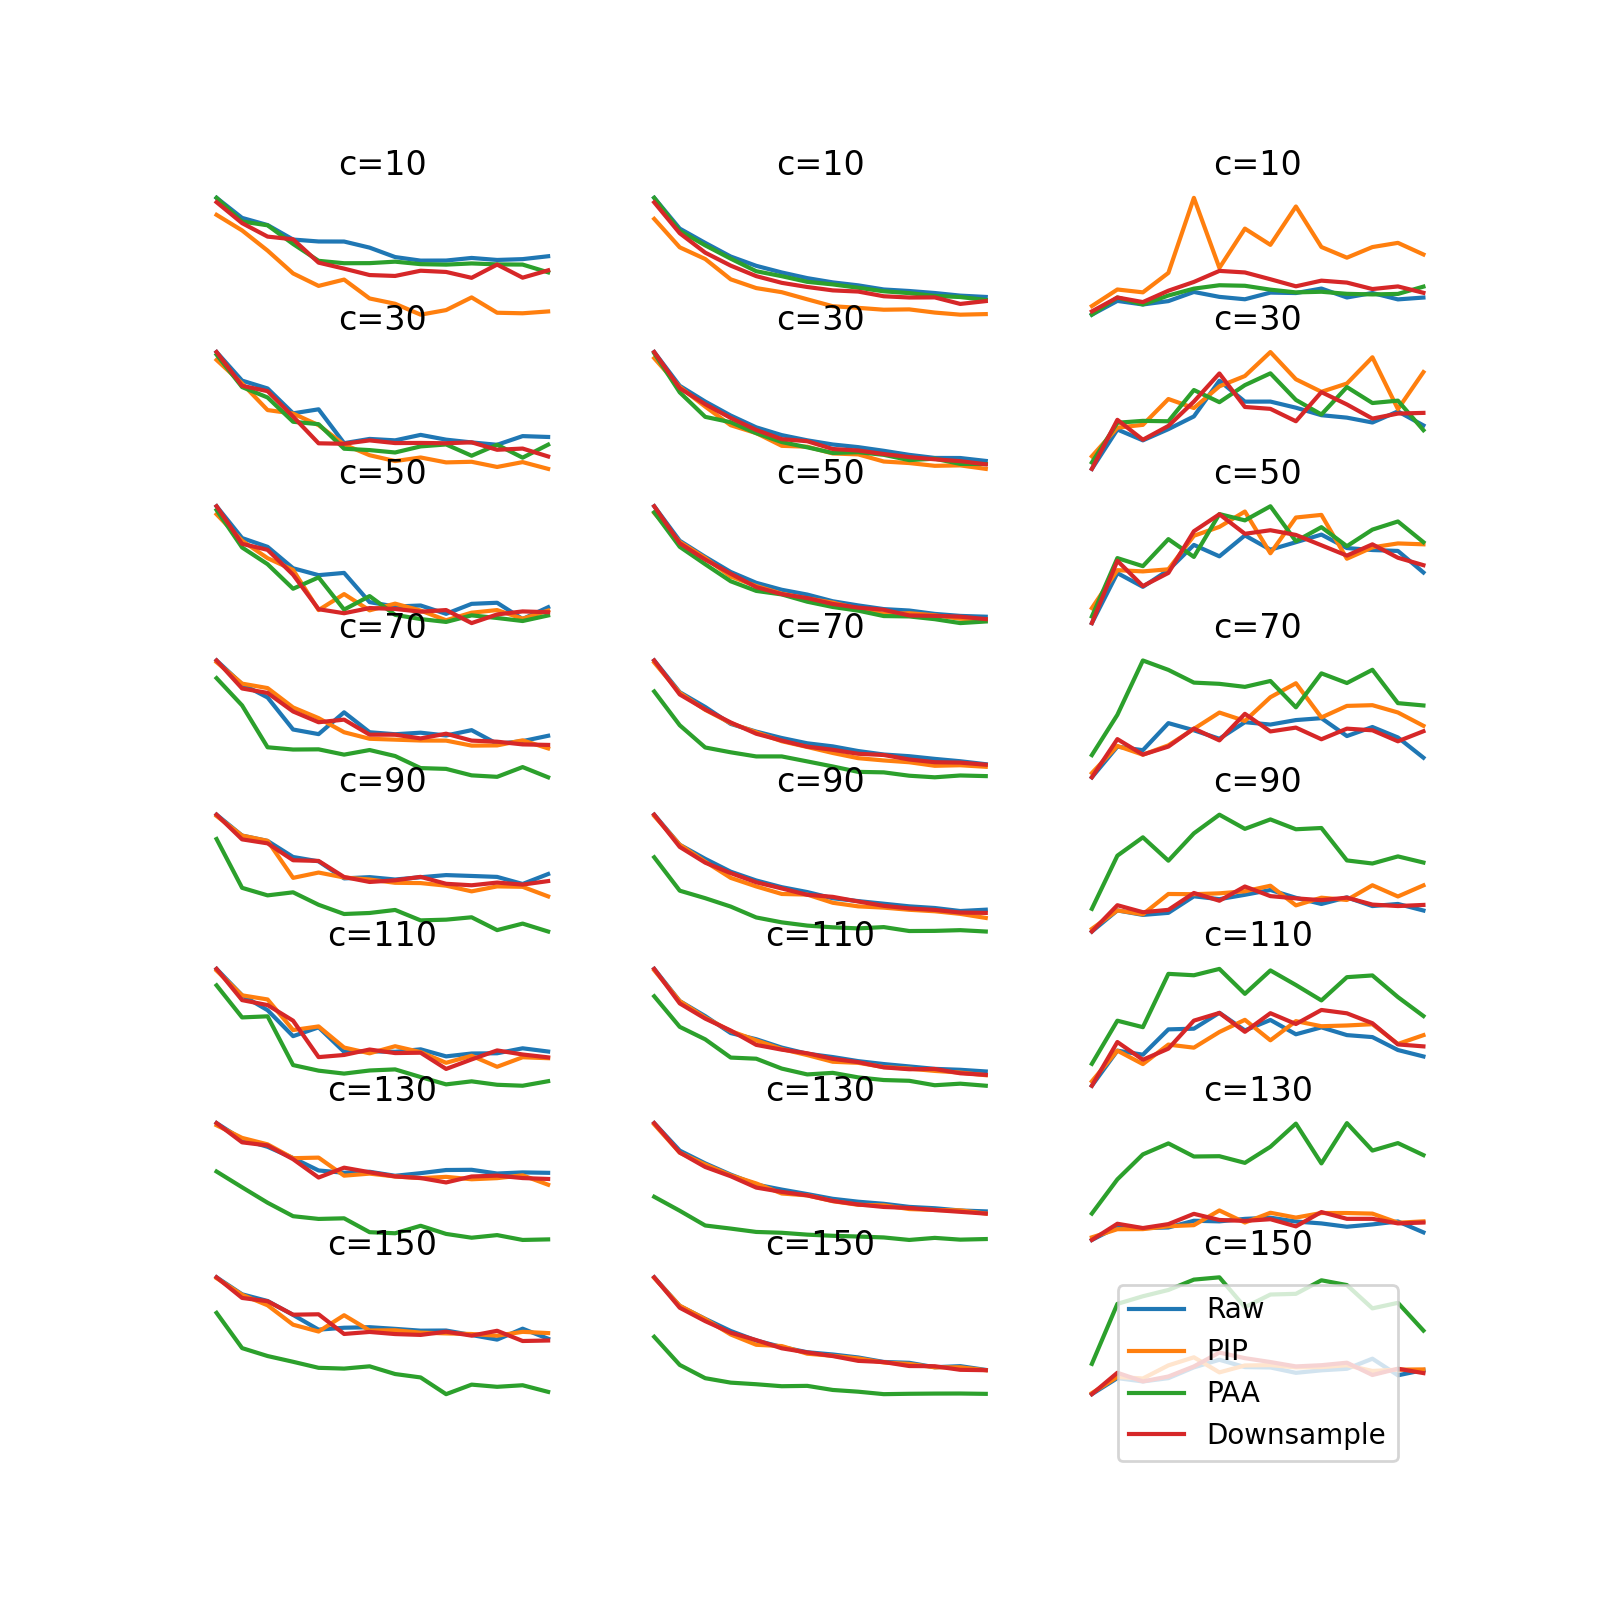
\includegraphics[width=0.3\columnwidth]{pippaac.png} 
    } 
    \subfigure[2012] { \label{fig:comparison2012} 
    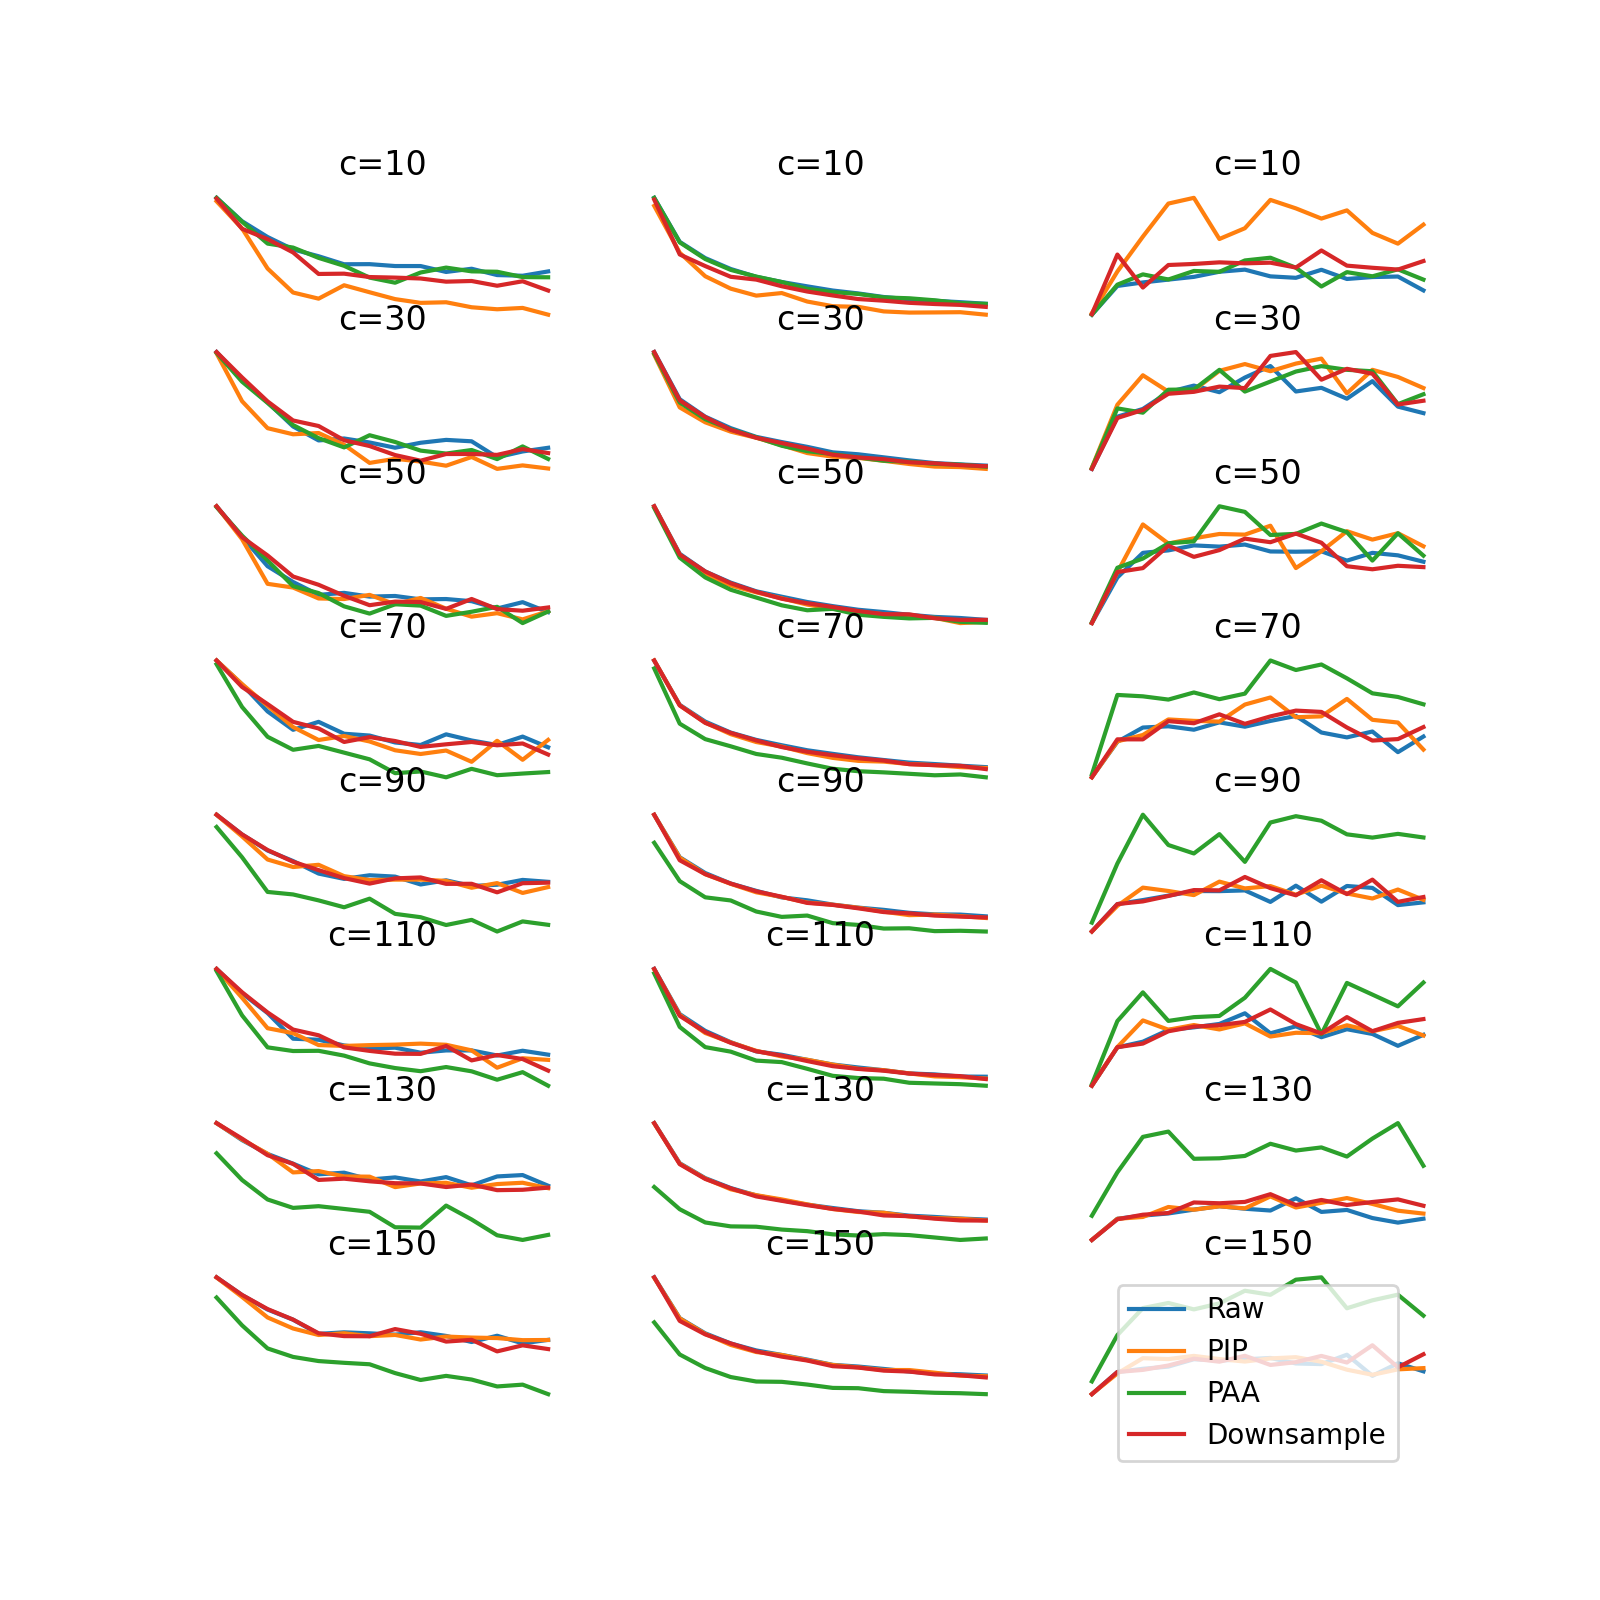
\includegraphics[width=0.3\columnwidth]{pippaac2012.png} 
    } 
    \subfigure[2013] { \label{fig:comparison2013} 
    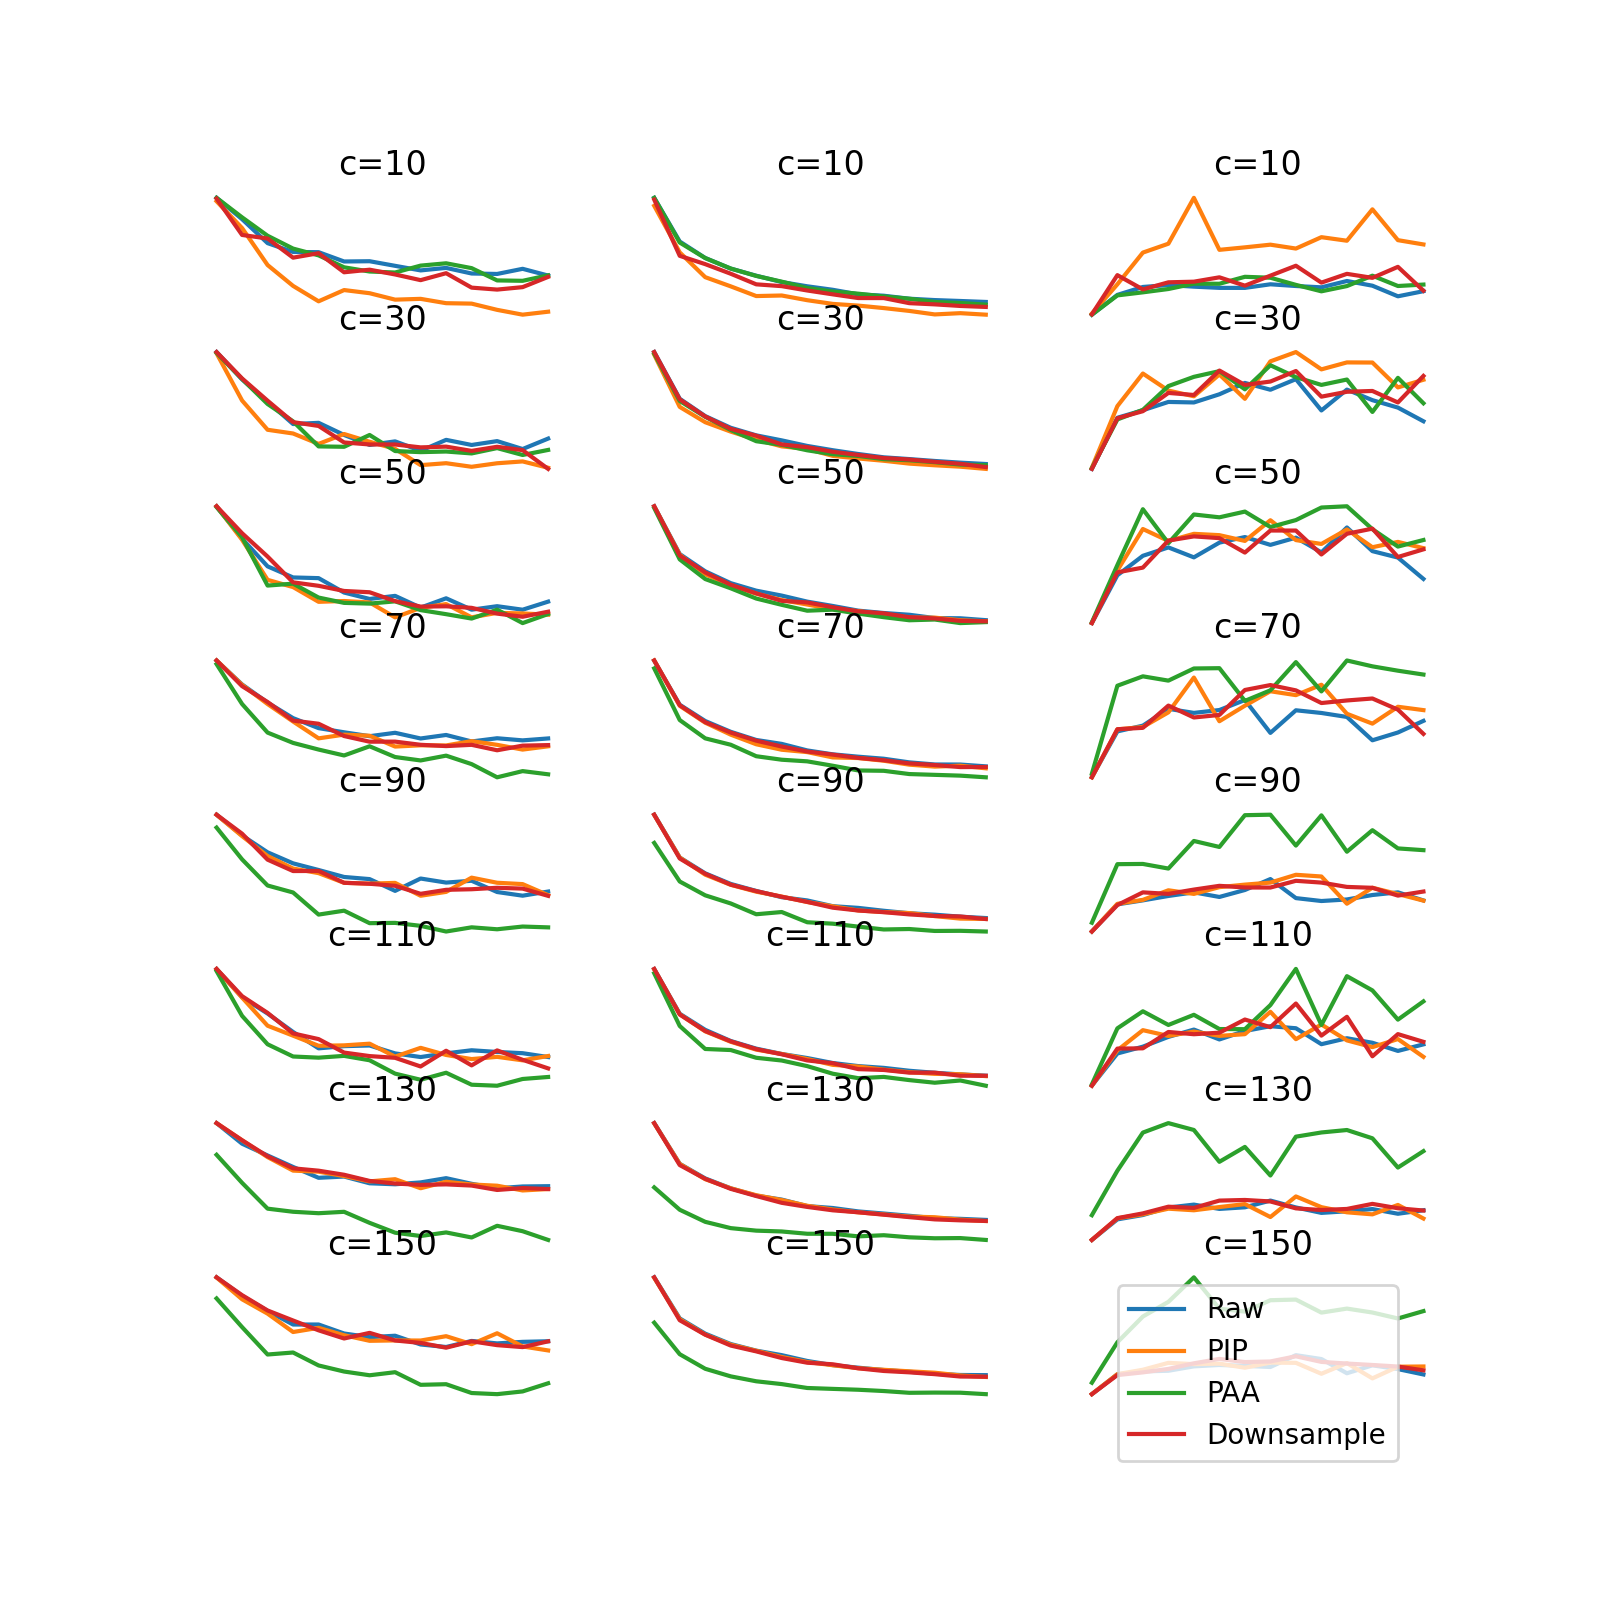
\includegraphics[width=0.3\columnwidth]{pippaac2013.png} 
    }
    \subfigure[2014] { \label{fig:comparison2014} 
    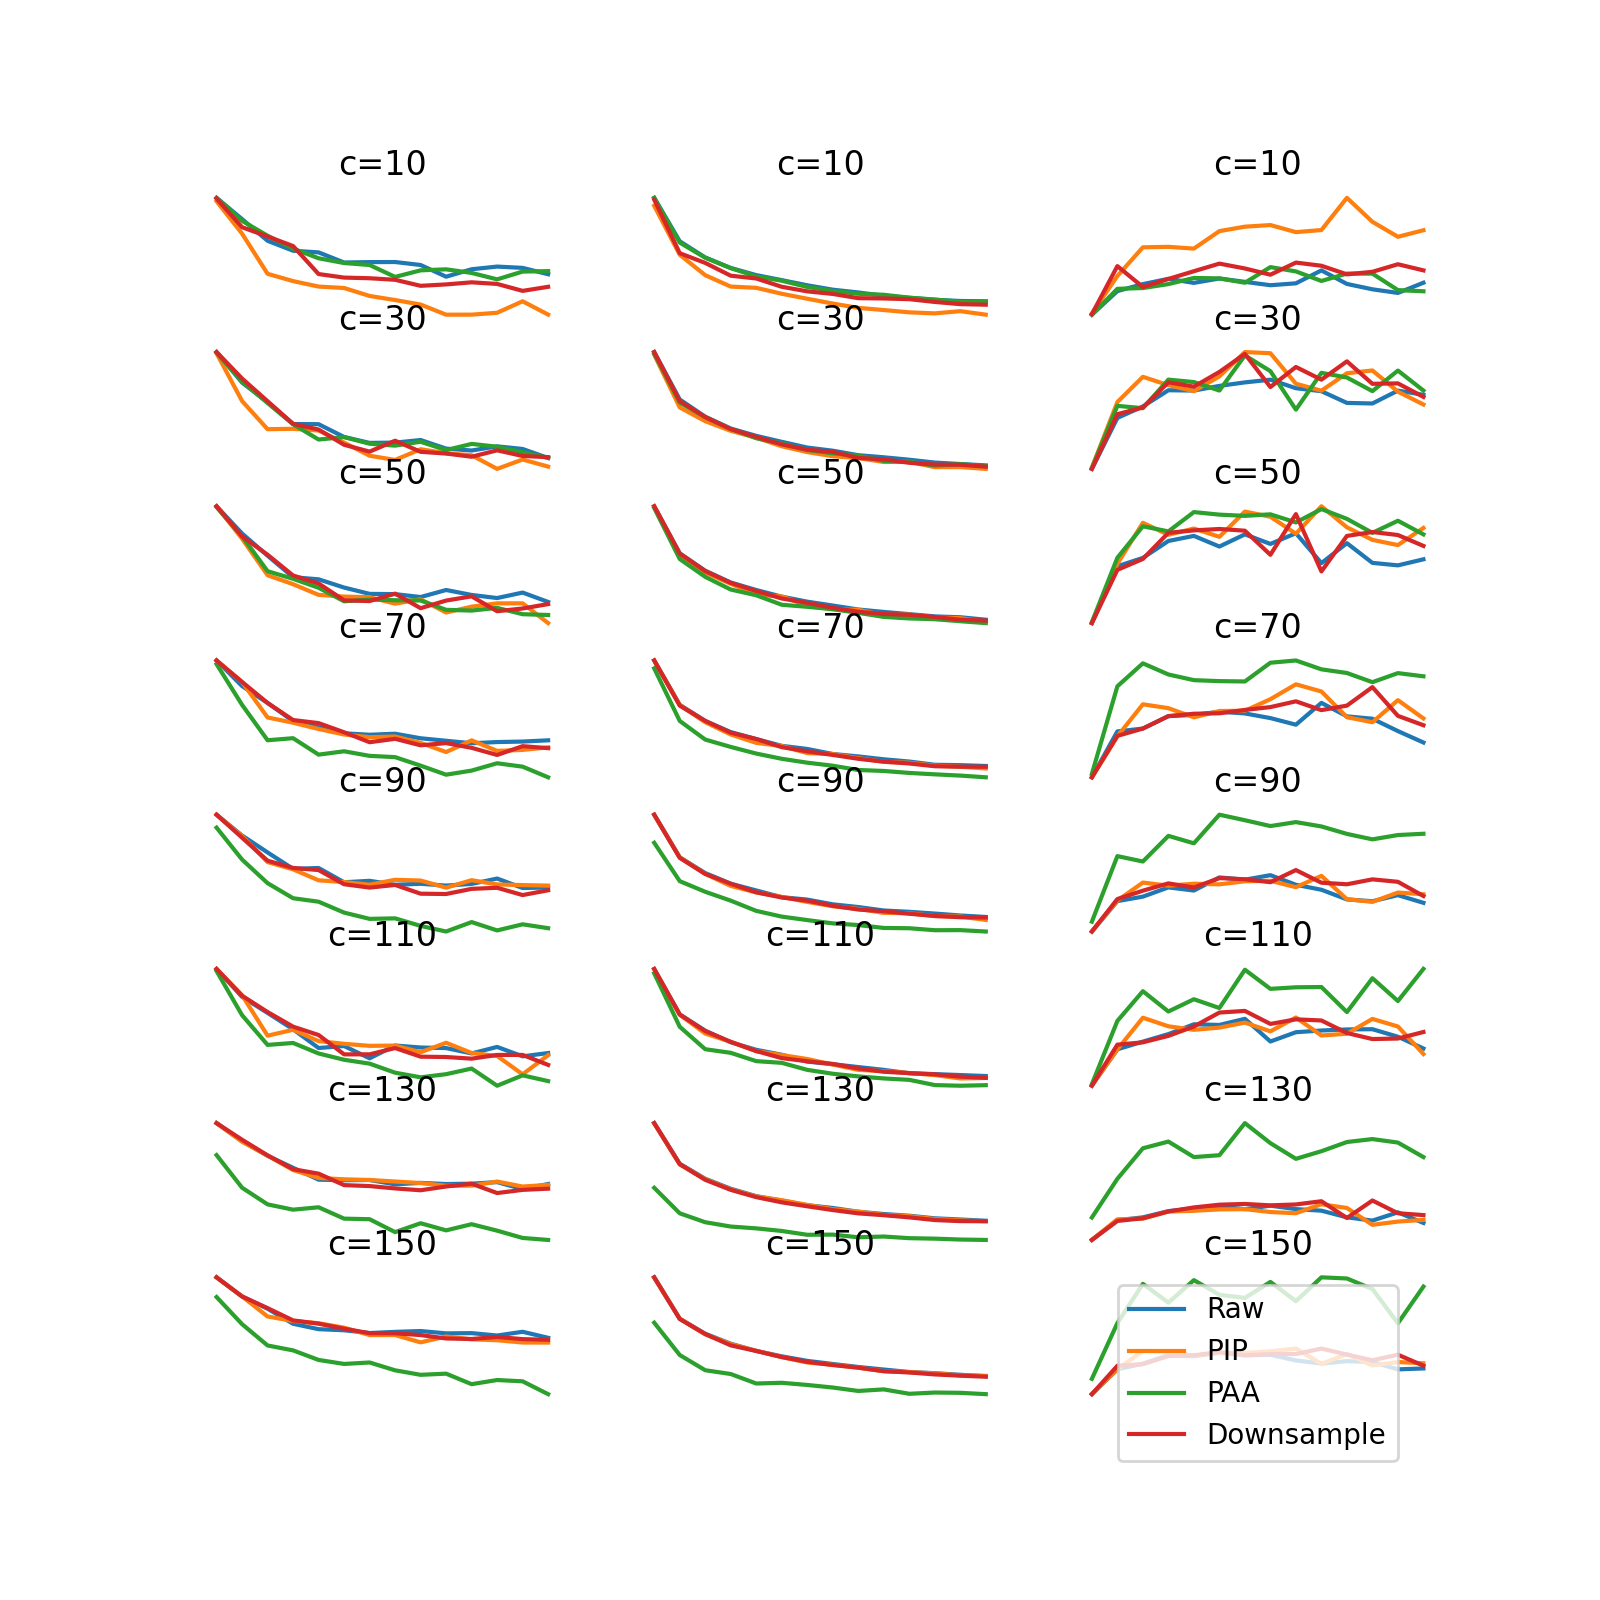
\includegraphics[width=0.3\columnwidth]{pippaac2014.png} 
    }
    \subfigure[2015] { \label{fig:comparison2015} 
    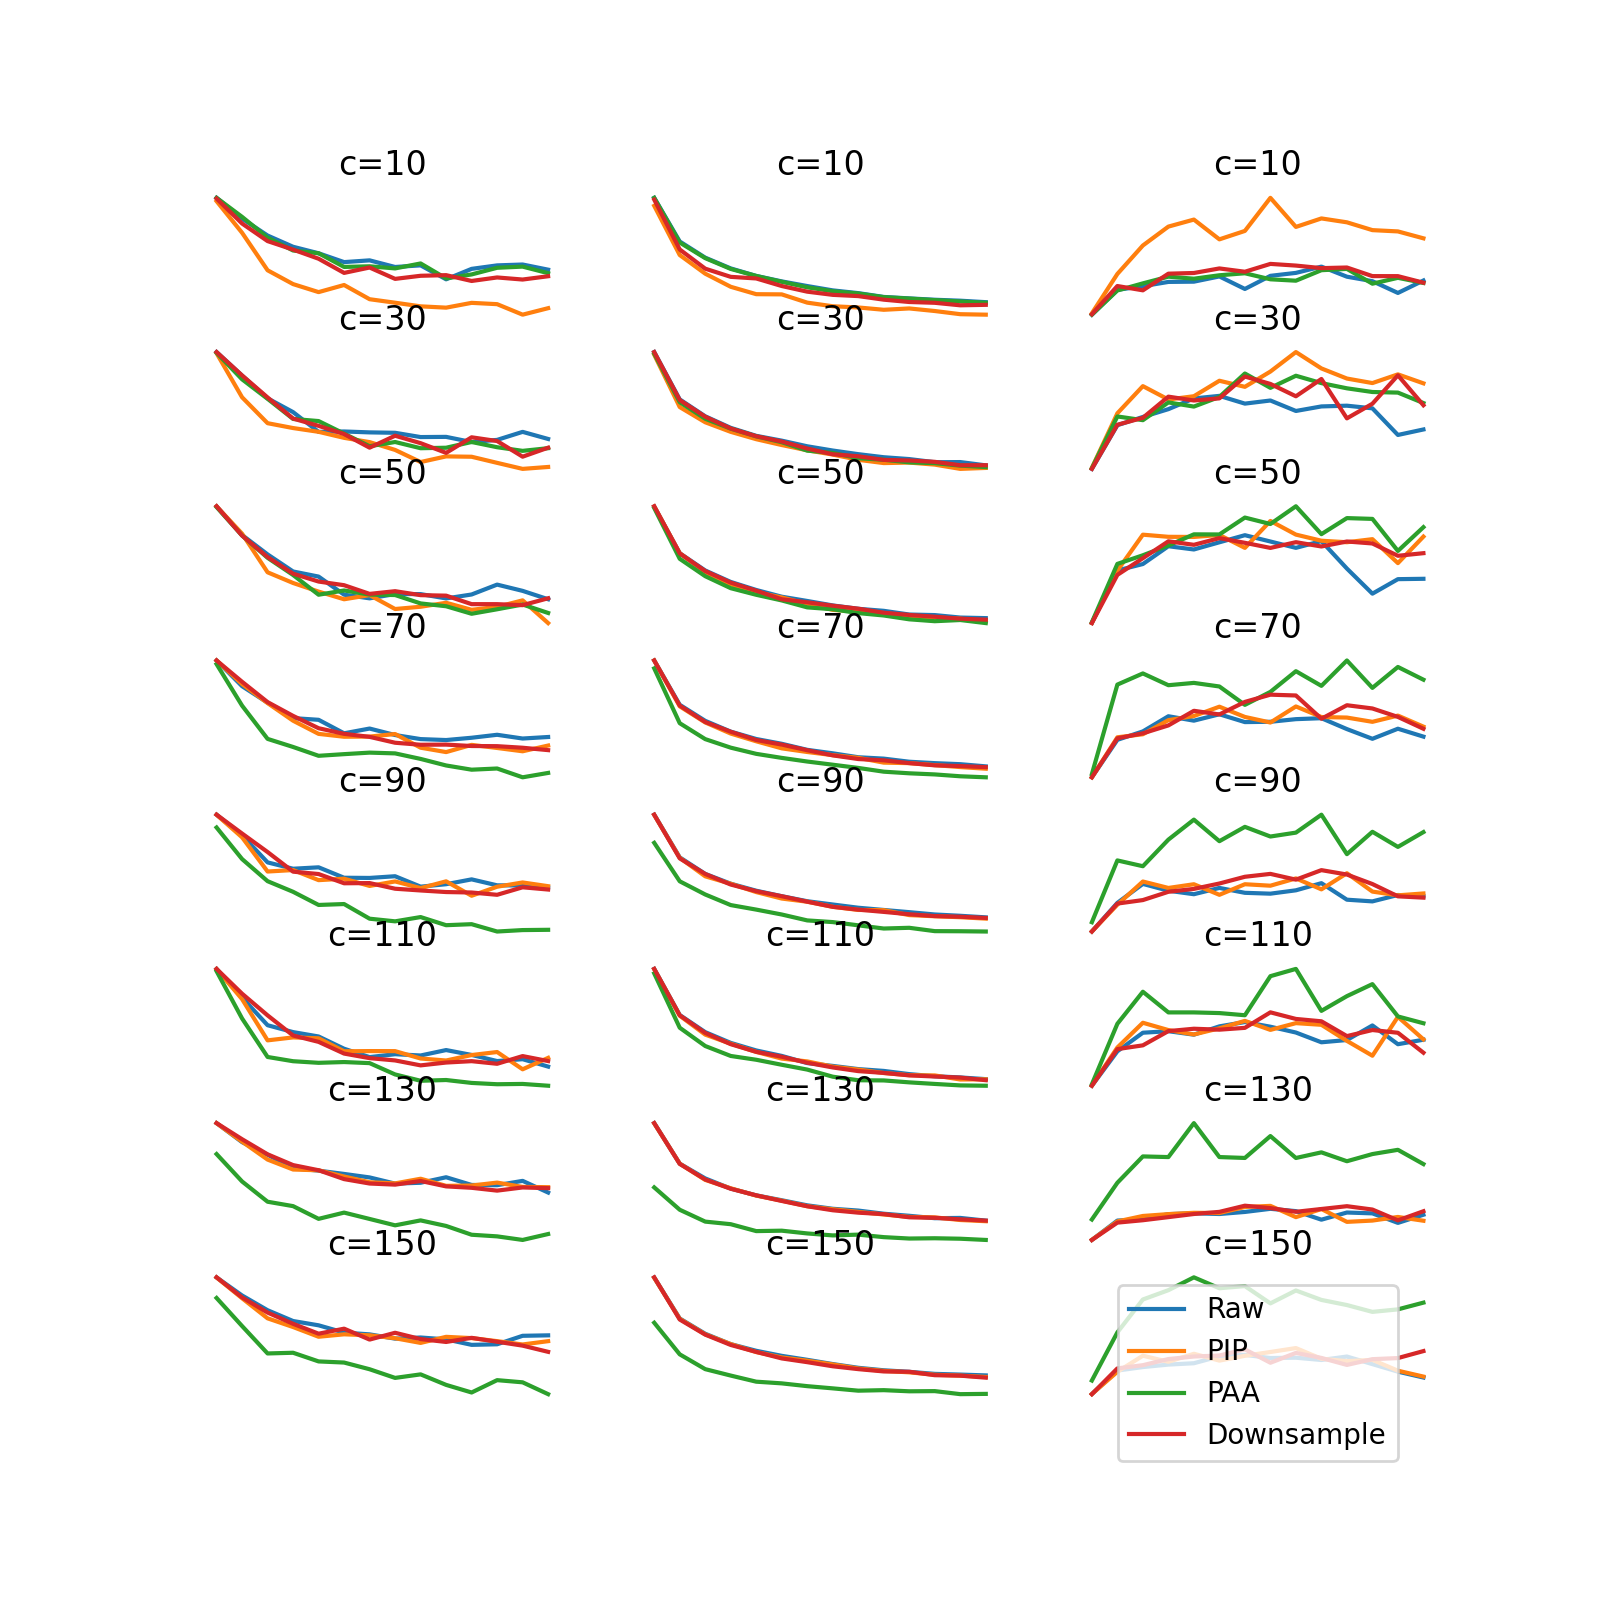
\includegraphics[width=0.3\columnwidth]{pippaac2015.png} 
    }
    \caption{ Different sequence length} 
    \label{fig:comparison1} 
\end{figure} 
\begin{figure}[!htbp]
    \centering 
    \subfigure[Raw 2011 (c=50)] { \label{fig:raw20111} 
    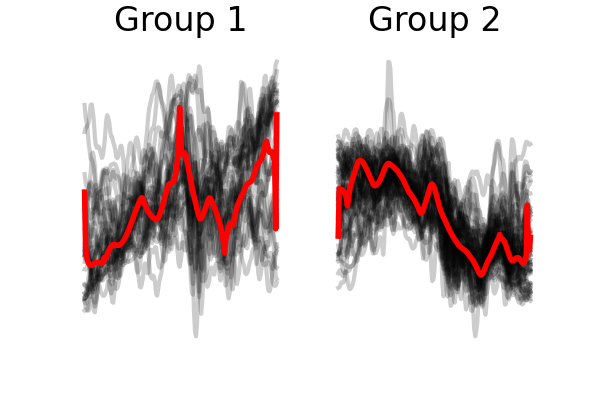
\includegraphics[width=0.4\columnwidth]{KshapeRaw1.png} 
    } 
    \subfigure[PIP 2011 (c=50)] { \label{fig:pip20111} 
    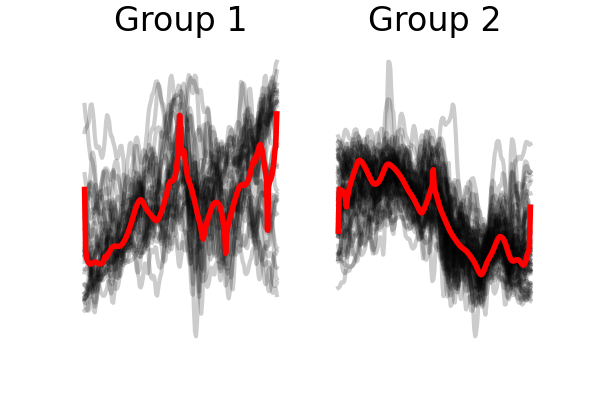
\includegraphics[width=0.4\columnwidth]{KshapePIP1.png} 
    }
    \subfigure[PAA 2011 (c=50)] { \label{fig:paa20111} 
    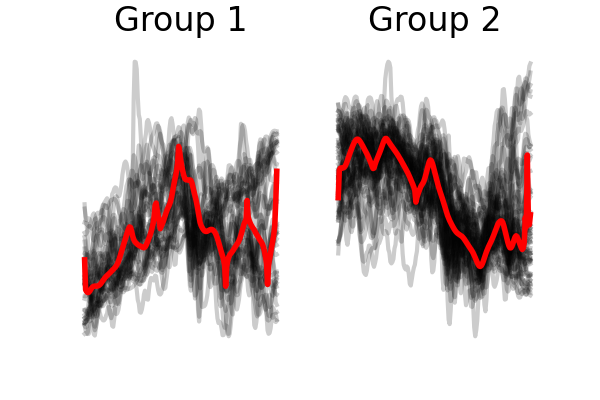
\includegraphics[width=0.4\columnwidth]{KshapePAA1.png} 
    }
    \subfigure[Downsampling 2011 (c=50)] { \label{fig:down20111} 
    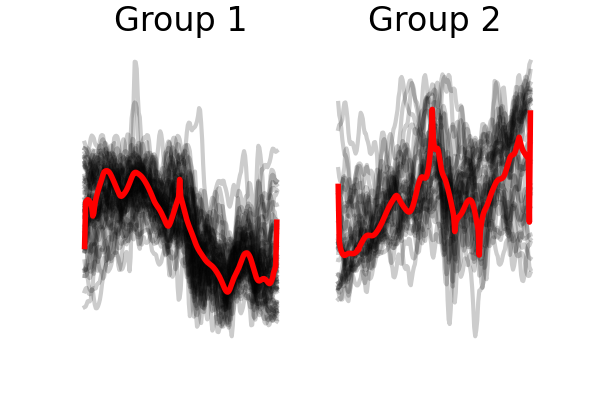
\includegraphics[width=0.4\columnwidth]{KShapedown1.png} 
    } 
    \caption{ Visual comparison } 
    \label{fig:pippaavisul} 
\end{figure} 
\\From those observations, we conclude there is no improvement of using compression in terms of these three indexes. However, take the execution time and the storage cost into consideration, the compressed version is at least linearly faster than original version while use less memory, which emphasizes the importance of compression in time-series clustering tasks. 